\usetikzlibrary{arrows.meta}
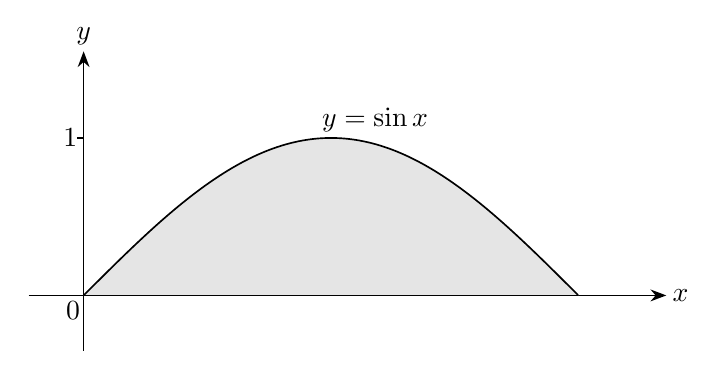
\begin{tikzpicture}[x=2cm,y=2cm,line width=.6pt,>=Stealth,font=\normalsize]
% axes math units: x in radians, y units
\draw[->] (-0.35,0)--(3.70,0) node[right,inner sep=0pt,xshift=2pt] {$x$};
\draw[->] (0,-0.35)--(0,1.55) node[above,inner sep=0pt,yshift=2pt] {$y$};
% origin and y=1 tick
\draw[line width=.6pt] (0,1)--(-0.04,1);
\node[anchor=east,inner sep=0pt,xshift=-2pt] at (0,1) {$1$};
\node[anchor=north east,inner sep=0pt,xshift=-1pt,yshift=-2pt] at (0,0) {$0$};
% shaded region under y=sin x on [0,pi]
\fill[gray!20] (0,0) -- plot[domain=0:3.14159265,samples=120] (\x,{sin(deg(\x))}) -- (3.14159265,0) -- cycle;
% curve y=sin x, exact formula
\draw[domain=0:3.14159265,samples=160] plot (\x,{sin(deg(\x))});
% vertical hatch strokes are represented by solid shading; redraw base segment
\draw (0,0)--(3.14159265,0);
% label above peak with clearance
\node[anchor=south,inner sep=0pt,yshift=4pt] at (1.85,0.96) {$y=\sin x$};
\end{tikzpicture}
